\documentclass[fontsize = 12pt, paper = a4]{scrreprt} 

\setlength{\parindent}{0pt}
\usepackage[english,ngerman]{babel}
\usepackage[utf8]{inputenc} 
\usepackage{enumerate}
\usepackage{amssymb,amsmath}

%------------ Überschriften verkleinern und hochsetzen ----------%

%\makeatlettern
%\renewcommand*\@makechapterhead[1]{%
%{\parindent \z@ \raggedright \normalfont
%\LARGE\bfseries
%\ifnum \c@secnumdepth >\m@ne
%\thechapter\space
%\fi
%#1\par\nobreak
%\vskip 20\p@
%}} 

% ------------------------ Blattlayout- -------------------------%

\usepackage {geometry}   
\geometry   {left     = 2.5cm,
             right    = 2.5cm, 
             top      = 1.5cm,
             bottom   = 1.5cm,
             includehead, includefoot}
             
% ------------------------ Seitenstil ---------------------------%           

% Umdefinieren von Befehlen zur Vermeidung von Bugs:

\renewcommand*{\chapterpagestyle}{scrheadings} 
\renewcommand*{\chapterheadstartvskip}{\vspace*{-\topskip}}

% Gestaltung der Kopf- und Fußzeile:

\pagenumbering{arabic}
            
\usepackage[automark]{scrpage2}
\automark[chapter]{section}
\pagestyle{scrheadings} 
\ohead[\pagemark]{\pagemark}
\setlength{\footskip}{5mm} 

\clearscrheadfoot
\lohead{Benutzerhandbuch}
\rohead{\headmark}
\lofoot{Softwareprojekt TU Ilmenau SS 2013}
\rofoot{\pagemark}

% Kopf- und Fußzeilenlinie:

\setheadsepline{.6pt} % Linie für Kopfzeile
\setfootsepline{.6pt} % Linie für Fußzeile 

% Für Unterstreichungen:

\usepackage[normalem]{ulem}

% Buchstabenglättung am Rand:
  
\usepackage {microtype} 

% Bildunterschriften zentrieren:

%\usepackage{caption}
%\captionsetup{margin=10pt,font=small,labelfont=bf, justification = centering}

%-------------------------------------------------------------------%

% Für die Einbindung von Bildern:

\usepackage[pdftex]{graphicx} % .pdf, .png oder .jpg möglich!
\usepackage{rotating}         % Grafiken rotieren

% Nutzung in drei Umgebungen möglich:

% (1) \begin{turn}{Winkel} ...  \end{turn}
% (2) \begin{sideways} ... \end{sideways} 90° im math. pos. Sinn
% (3) \begin{rotate}{Winkel} ... \end{rotate} 
%     ---> 90° im math. pos. Sinn, allerdings keine Platzreservierung 

\usepackage{wrapfig}
%\usepackage{picins}   % Textumflossene Grafiken
\usepackage{subfigure}
\usepackage{floatflt}
\usepackage[justification=centering]{caption}

%-------------------------------------------------------------------%
 
% Packete für Tabellen:

\usepackage{booktabs}
\usepackage{array}    % optional
\usepackage{tabularx} % optional

\usepackage[font=footnotesize,labelfont=bf,singlelinecheck=false,
            format=plain,,justification=justified,indention=0cm]                     {caption} 

\usepackage{setspace}

%----------------  Anfang des Dokuments ------------------%

\begin{document}

%*******************************************************************%

% Entwurf Titelseite:

\titlehead{\begin{center}
\textbf{\Huge Entwurfsdokument}
\end{center}}
		   
\title{Service-Interface \\ für ein Formula-Student-Fahrzeug}

\subtitle{Technische Universität Ilmenau \\
		  Softwareprojekt SS 2013 \\ Gruppe 19}			
		
\author{Christian Boxdörfer \\ Thomas Golda \\ Daniel Häger \\ 
		David Kudlek \\  Tom Porzig \\ Tino Tausch \\ 
		Tobias Zehner \\ Sebastian Zehnter}
		
\date{Hier Datum einfügen}	 
	  
\publishers{betreut durch \\ \vspace{1cm} Dr. Heinz-Dietrich Wuttke, TU Ilmenau \\ Oliver Dittrich, fachlicher Betreuer Team StarCraft e.V.}

\maketitle		

%*******************************************************************%

% --------------------- Inhaltsverzeichnis -----------------------%

\begin{spacing}{0.86} 
\tableofcontents
%\setcounter{secnumdepth}{4} % Tiefere Gliederungsebene  
\setcounter{tocdepth}{4} % Anzeige bis Gliederungsstufe 4
%\addtocontents{toc}{\protect\enlargethispage{2\baselineskip}} 
\end{spacing}


\newpage % Seitenumbruch

%--------------------------  Einleitung  ---------------------------%

\chapter{Einleitung}

%----- Installation und Konfiguration des Service Interfaces -------%

\chapter{Installation und Konfiguration des Service Interfaces}


%-------------------------------------------------------------------%
%-------------------------------------------------------------------%

\section{MicroAutoBox II}

Für eine erfolgreiche Installation und Konfiguration der MicroAutoBox II müssen zu Beginn der Installation neben dieser Hardwarekomponente folgende Dateien in MATLAB und Modelle in Simulink vorliegen:

\begin{itemize}

\item \textit{udp\_final.mdl}: Diese Datei beinhaltet das von uns bereitgestellte Simulink-Modell für das Service Interface.

\item \textit{config\_datenpaket.m} Dieses *.m - File enthält die zur Konfiguration des Datenpaketes notwendigen Vektoren, welche je nach Art des Datenpaketes an dieses angepasst werden können und Informationen über dessen Attribute und Zusammensetzung beinhalten (Verweis ED).

\item \textit{signalgenerator\_microautobox.m} Dieses optionale *.m - File dient dazu, den Signalgenerator im Simulink-Modell zu Simulationszwecken mit generierten Testdaten auszustatten, um bei Veränderungen des Simulink-Modells oder bei einer Modifizierung der   auf dem Embedded-PC oder dem virtuellen Server implementierten *.cpp - Dateien eine Verifizierung des Service Interfaces anhand dieser bekannten Testdaten durchführen zu können (Verweis ED).

\end{itemize} 

Falls diese Dateien alle zur Verfügung stehen sollten, ist in einem ersten Schritt das Simulink-Modell \textit{udp\_final.mdl} durch das Programm MATLAB zu öffnen, wonach sich in Simulink auf der obersten Modellebene  folgende Subsysteme befinden (s. Abb. \ref{topmodell}):

\begin{figure}[h]
\centering
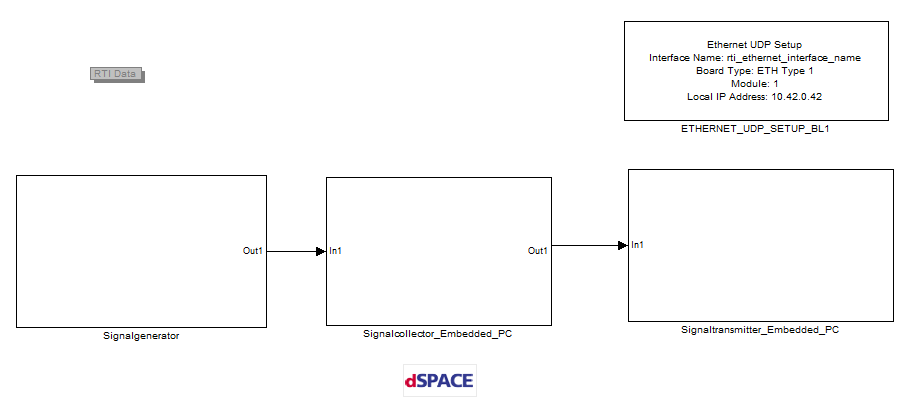
\includegraphics[scale = 0.65]{topmodell}
\caption[Gesamtaufbau Simulink-Modell]{Gesamtaufbau des Simulink-Modells auf höchster Modellebene}
\label{topmodell}
\end{figure} 

\newpage

%-------------------------------------------------------------------%

\subsection{Konfiguration der Ethernet-Schnittstelle}

Daraufhin ist bei der weiteren Vorgehensweise anschließend die Konfiguration der Ethernet-Schnittstelle vorzunehmen. Hierzu öffnet man durch einen Doppelklick den in Abb. \ref{topmodell} zu sehenden Block \textit{"`Ethernet UDP Setup"} ein Fenster, in welchem nun die Möglichkeit besteht, zwischen den beiden Reitern \textit{"`Unit"} und \textit{"`Options"} zu navigieren (Verweis dSPACE Doku) und dort bei den jeweiligen Einstellungen Modifikationen vorzunehmen. Im Folgenden werden obligatorische Änderungen durch ein (*) am jeweiligen Parameter gekennzeichnet. \\

\textbf{Reiter "`Unit"} 

\begin{itemize}

\item \textit{Interface Name}: Hier kann ein selbst gewählter Name für die Schnittstelle festgelegt werden.

\item \textit{$Board \ Type \ ^{(*)}$}: Bei Verwendung der MicroAutoBox II ist dort die Option \\ "`ETH Type 1"\ auszuwählen.

\item \textit{Module number}: Der dortige Wert ist auf "`1" vorkonfiguriert und kann auch so belassen werden.

\item \textit{$Local \ IP \ adress \ ^{(*)}$}: Hier ist die lokale IP-Adresse der MicroAutoBox II in Abhängigkeit vom gewählten Subnetz  anzugeben (z.B. 192.X oder 10.X).

\end{itemize}

\textbf{Reiter "`Options"} \\

In diesem Reiter können anhand nachfolgender Einstellungen bis zu vier verschiedene Sockets innerhalb des Modells definiert werden. Der Socket 1 ist hierbei für das Datenpaket mit den Fahrzeugdaten und Socket 2 für das Datenpaket mit den Paketinformationen vorgesehen. Darüber hinaus stehen bei beabsichtigten Erweiterungen des Modells Socket 3 und 4 zur freien Verfügung.

\begin{itemize}

\item \textit{$Enable \ ^{(*)}$}: Ein gesetztes Häkchen entscheidet bei diesem Parameter darüber, ob der jeweilige Socket aktiviert oder deaktiviert wird. Es ist notwendig, die Sockets 1 und 2 zu aktivieren, um den Transport der Datenpakete an den Embedded-PC zu ermöglichen (s. o.). Darüber hinaus sollten die Sockets 3 und 4, falls diese nicht anderweitig verwendet werden, deaktiviert werden.  

\item \textit{$Local \ Port \ Number \ [0 \ ... \ 65535] \ ^{(*)}$}: In diesem Feld ist die Nummer des lokalen Ports der MicroAutoBox II einzutragen. 

\item \textit{$Remote \ Port \ Number \ [0 \ ... \ 65535] \ ^{(*)}$}:
Dort muss die Nummer des externen Ports -- also der gewünschte Port des Embedded-PCs -- eingetragen werden. \\ Anmerkung: Um Verwechslungen beim Eintragen der Portnummern o.ä. zu vermeiden, ist es empfehlenswert, für beide Ports die selbe Nummer zu vergeben. 

\end{itemize} 

Nachdem alle obligatorischen Änderungen vorgenommen wurden, muss in einem nächsten Schritt innerhalb der Subsysteme \textit{UDP\_DATEN} und \textit{UDP\_PAKETINFORMATIONEN} die Blöcke "`ETHERNET\_UDP\_TX\_BL1"\ und "`ETHERNET\_UDP\_TX\_BL2"\ angepasst werden.

\newpage

%-------------------------------------------------------------------%

\subsection{Konfiguration der Matlabfiles \textit{signalgenerator\_microautobox.m} und \textit{config\_datenpaket.m}}

%-------------------------------------------------------------------%

Abhängig von den weiteren Absichten des Benutzers werden im Folgenden nun für diese Ziele die jeweiligen Vorgehensweisen ausführlich erläutert. 

\subsection{Testen des Simulink-Modells durch den Signalgenerator}

%-------------------------------------------------------------------%


\subsection{Anschluss des Simulink-Modells des Formula-Student-Fahrzeuges an das Simulink-Modell des Service Interfaces}

%-------------------------------------------------------------------%

\subsection{Implementierung des Modells auf der MicroAutoBox II}

%-------------------------------------------------------------------%

\subsection{Appendix: Hinzufügen, Entfernen oder Modifizieren von Signalen}

%-------------------------------------------------------------------%




\section{Embedded-PC}

\section{vServer}

\section{Datenbanken}

\subsection{Fahrzeugdatenbank}

\subsection{Benutzerdatenbank}

\section{Webseite}

%----------------- Bedienung des Service-Interfaces ----------------%

\chapter{Bedienung des Service-Interfaces}


\end{document}